% Chapter Template

\chapter{Estado del Arte} % Main chapter title

\label{Chapter2} % Change X to a consecutive number; for referencing this chapter elsewhere, use \ref{ChapterX}

%----------------------------------------------------------------------------------------
%	SECTION 1
%----------------------------------------------------------------------------------------

\section{An\'alisis de im\'agenes de la retina}

El an\'alisis de im\'agenes de la retina es de gran importancia para la detecci\'on de enfermedades del ojo.
El avance tecnol\'ogico permiti\'o obtener im\'agenes de la retina con mayor calidad, lo que beneficia la detecci\'on precoz de enfermedades con mayor precisi\'on, favoreciendo la disminuci\'on del porcentaje de personas con ceguera debido a enfermedades sistemicas o retinales. 

%-----------------------------------
%	SUBSECTION 1
%-----------------------------------
\subsection{Introducci\'on}

Durante la \'ultima d\'ecada, la fotograf\'ia digital a color ha sido reconocida como una modalidad aceptable para documentar el aspecto de la retina, ya que proporciona informaci\'on vital sobre la salud del paciente de la parte sensorial del sistema visual. La segmentaci\'on y el an\'alisis de im\'agenes autom\'aticas de la retina se pueden utilizar para detectar el riesgo patol\'ogico o da\~nos, y para ayudar en el diagn\'ostico. 

T\'ecnicas de procesamiento de imágenes, análisis y visión por ordenador se encuentran hoy en d\'ia en todos los campos de la ciencia m\'edica. Estas técnicas son especialmente relevantes para la oftalmología moderna, un campo que depende en gran medida de los datos visuales. Las im\'agenes de la retina son ampliamente utilizadas por ofatalm\'ologos para fines de diagn\'ostico. Sin embargo, estas im\'agenes a menudo necesitan mejora visual antes de determinar un an\'alisis digital de riesgo patol\'ogico o la detecci\'on de da\~nos.

Lo anterior referencia a -> Marrugo2011

Se prevee que la Diabetes Mellitus (DM) llegue a 600 millones de personas en el mundo en 2035, generando tambi\'en una posible epidemia en Asia.
La retinopat\'ia diab\'etica (DR), una complicaci\'on de la DM, afecta a un tercio de los diab\'eticos  y es la principal causa de p\'erdida de visi\'on en personas de edad avanzada,  y sigue siendo una de las principales causas de ceguera evitable. El edema macular diab\'etico (DME), caracterizado por el aumento de la permeabilidad vascular y la deposici\'on de exudados duros en la retina central, puede desarrollarse en cualquier etapa de la DR y aflige a 21 millones de personas en el mundo.

A trav\'es de ex\'amenes peri\'odicos de la vista, la p\'erdida de la visi\'on relacionada con la diabetes se puede prevenir en el 98\% de los casos.

Lo anterior referencia a -> g0h2016

La retina es un tejido en capas que recubre el interior del ojo, permitiendo la conversión de la luz entrante en señales neuronales adecuadas para su posterior procesamiento por parte de la corteza visual del cerebro. La misma está sostenida por el epitelio pigmentario retinal, la coroide y la esclera.

La estructura anatómica del ojo se compone básicamente por la córnea (transparente), la esclera (normalmente blanca), el iris (que da color al ojo) y la pupila. Todas estas partes son visibles desde el exterior, y son las responsables de permitir la visión: un rayo de luz pasa a través de la córnea, que enfoca parcialmente la imagen, luego pasa por la cámara anterior, la pupila (que hace las veces de lente y enfoca aún más la imagen), la vítrea y por último es enfocado en la retina.

VA LA IMAGEN DEL OJO CON SUS PARTES


Actualmente existen diversas \'areas de investigación activas en lo que respecta a la imagenología de la retina. Algunas de las \'areas se centran en la b\'usqueda de herramientas t\'ecnicas rentables, f\'aciles de usar y portables. Por otro lado CONSULTAR IMAGENES FUNCIONALES. Otra \'area (Adaptive Optics) se encarga de la utilizaci\'on de lentes para corregir las fallas de frente de onda de la luz reflejada desde la retina, permitiendo la obtenci\'on de celulas individuales o estructuras celulares.
Longer Wavelength OCT Imaging realiza investigaciones para el desarrollo de los l\'aseres de baja coherencia de c\'odigo de barrido con longitudes de ondas centrales mayores. Algunos de estos prototipos ya son capaces de resolver los detalles en la coroides y la l\'amina cribosa.






%-----------------------------------
%	SUBSECTION 2
%-----------------------------------

\subsection{Fotograf\'ias de fondo de ojo}

El Instituto Nacional del Reino Unido (NICE) establece que una prueba de cribado de RD debe tener la sensibilidad y la especificidad de al menos el 80\% y 95\%, respectivamente, con una tasa de fallo t\'ecnico inferior al 5\%. El m\'etodo de la fotograf\'ia est\'andar para la detecci\'on de DR es la fotograf\'ia en color de fondo de ojo estereosc\'opica en 7 campos (30$^{\circ}$) definidas por el grupo de tratamiento temprano de la retinopat\'ia diab\'etica Study (ETDRS). También es \'util para la identificaci\'on de DME y la neovascularizaci\'on retinal sutil. Sin embargo, desde la perspectiva del paciente, teniendo 7 campos es mucho tiempo, tediosa e inc\'omoda.
Actualmente se utilizan  2 o 3 campos para el cribado en la fotograf\'ia de fondo de ojo, ya que representan un compromiso razonable de la sensibilidad y buena  comodidad para el paciente.
La fotograf\'ia de fondo midr\'iatico ha demostrado ser una estrat\'egia eficaz de cribado de DR. Ofrece una sensibilidad de al menos 80\% en la detecci\'on de cualquier grado de DR, y la sensibilidad y especificidad de 97\% y 92\%, respectivamente,

El uso de sistemas de im\'agenes digitales ha reducido la tasa de fallo t\'ecnico asociado con la fotograf\'ia de pel\'icula anterior no digital, y la imagen electr\'onica que permite un f\'acil almacenamiento y catalogaci\'on. Los sistemas digitales modernos utilizados en la fotograf\'ia de fondo de ojo han demostrado lograr una sensibilidad y especificidad de aproximadamente el 90\% en la detecci\'on de DR.

Lo anterior referencia a -> g0h2016

Existen diversas formas de poder observar y analizar la anatom\'ia del ojo, a trav\'es de im\'agenes m\'edicas. 
Una de las modalidades de imagen m\'edica que permite explorar el interior del ojo es la de la imagen de fondo de ojo. La misma consiste en  una representaci\'on 2D del tejido retinal semitransparente 3D, proyectado en el plano de obtenci\'on de la imagen, que se obtiene usando la luz reflejada en el tejido.

Para realizar la captura del fondo de ojo, se dilata la pupila con f\'armacos que se depositan en forma de gotas en la superficie ocular; as\'i, el oftalm\'ologo puede ver con facilidad el interior del globo ocular con un aparato que se llama oftalmoscopio. El oftalmoscopio consiste en un aparato formado por una serie de espejos y cristales que alumbran la retina del ojo sin que la luz se refleje. Si no fuese por el oftalmoscopio la luz provocar\'ia destellos y no se podría ver el fondo de ojo de manera correcta, algo parecido a lo que sucede cuando el flash de una cámara de fotos saca los ojos en color rojo. Esta modalidad no es invasiva, y su costo es menor a la angiografía y la OCT dado que la c\'amara que se necesita para capturar la imagen del ojo es una c\'amara digital convencional.
Adem\'as de facilitar la detecci\'on de enfermedades oculares, las im\'agenes de fondo de ojo permiten detectar tres tipos de lesiones oculares. 


\begin{figure}[h]
%\centering
\minipage{0.32\textwidth}
	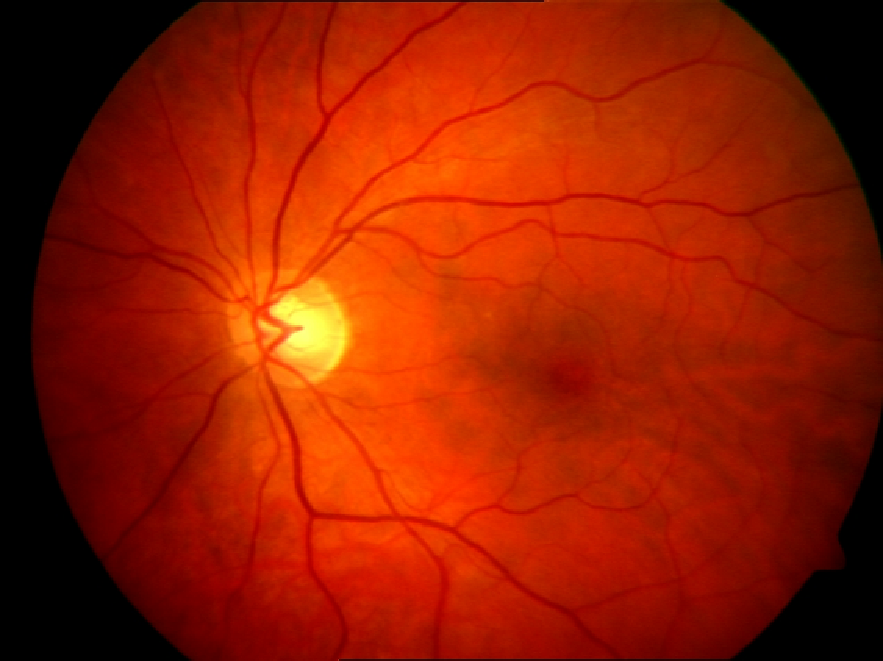
\includegraphics[width=\linewidth]{Figures/images}
	\caption[HRF]{HRF (Degeneración macular).}\label{fig:HRF}
\endminipage\hfill
%\decoRule
%\caption[HRF]{HRF (Degeneración macular).}
\minipage{0.32\textwidth}
	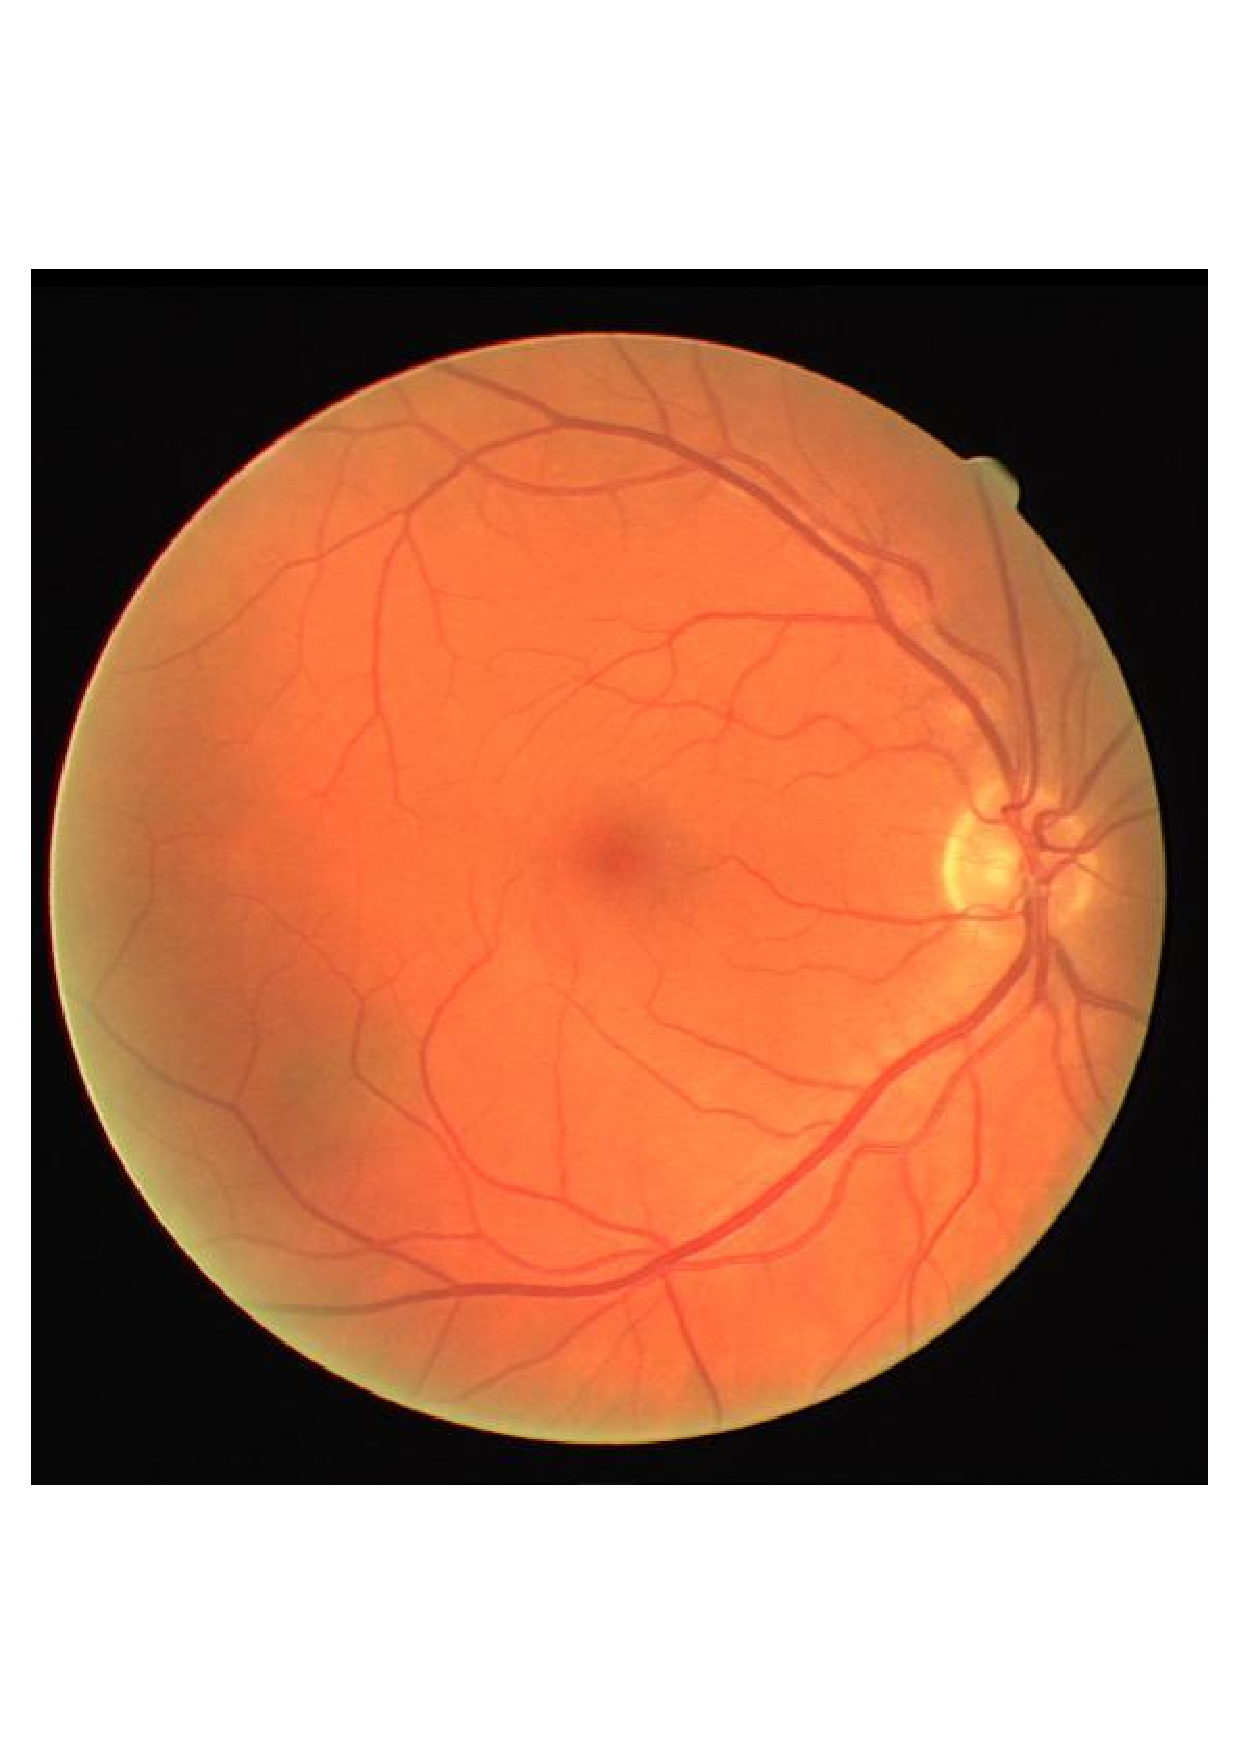
\includegraphics[width=\linewidth]{Figures/images1}
	\caption[ARIA]{ARIA (Degeneración macular).}\label{fig:ARIA}
\endminipage\hfill
\minipage{0.32\textwidth}
	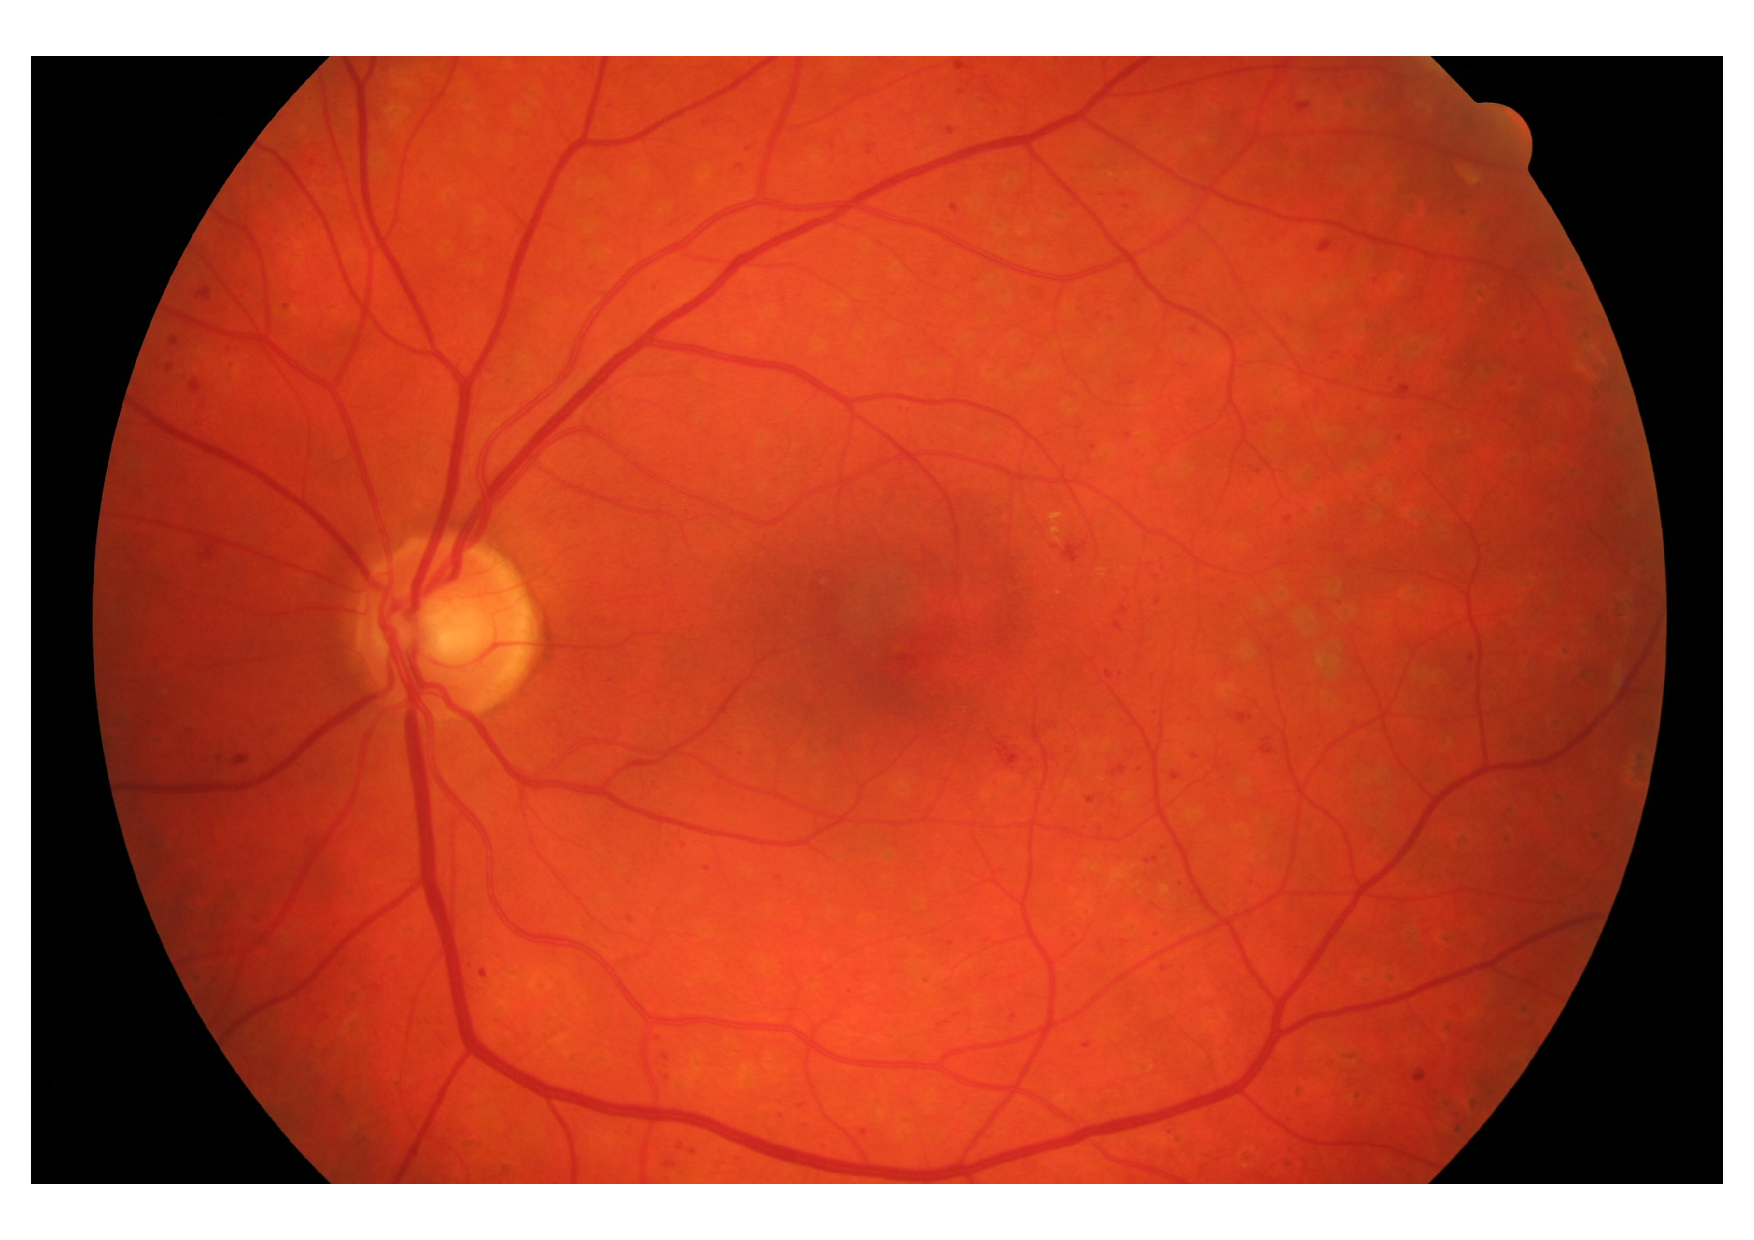
\includegraphics[width=\linewidth]{Figures/images2}
	\caption[HRF]{HRF (Degeneración macular).}\label{fig:HRF}
\endminipage\hfill

%\label{fig:Electron}
\end{figure}


%-----------------------------------
%	SUBSECTION 3
%-----------------------------------

\subsection{Herramientas computacionales para an\'alisis de fotograf\'ias de fondo de ojo}

%----------------------------------------------------------------------------------------
%	SECTION 2
%----------------------------------------------------------------------------------------

\section{Segmentaci\'on de vasos sangu\'ineos en im\'agenes de fondo de ojo}


%-----------------------------------
%	SUBSECTION 1
%-----------------------------------

\subsection{Necesidad}

%-----------------------------------
%	SUBSECTION 2
%-----------------------------------

\subsection{M\'etodos existentes}
